\section{Fondamenti di ML}

ML è un campo di studi che permette al computer di imparare dai dati senza essere esplicitamente programmato.

Un sistema ML si allena sulla task, non è esplicitamente programmato.

L'esperienza in ML sono i dati, che vengono presentati come esempio.

Le tasks del ML sono solitamente descritte su come il sistema di ML processa i dati.

Tipicamente si rappresentano gli esempio come vettori, dove ogni features dell'esempio è una entry del vettore.

\subsection{Tipologie di task}
\subsubsection{Classificazione}
Durante la classificazione, al sistema viene chiesto di capire a quale delle k categorie, l'input appartiene.


\begin{figure}[h!]
    \centering
    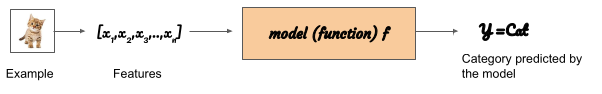
\includegraphics[width=0.6\linewidth]{imgs/15---classificazione-gatto}
    \caption{Esempio classificazione gatto}
    \label{fig:classificazione_gatto}
\end{figure}


\subsubsection{Regressione}
Al sistema viene chiesto di predirre un numero dati degli input.


\begin{figure}[H]
    \centering
    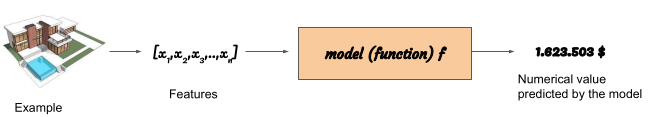
\includegraphics[width=0.6\linewidth]{imgs/16---regression}
    \caption{Esempio regressione}
    \label{fig:regressione}
\end{figure}


\subsubsection{Clustering}
Al sistema viene chiesto di ragruppare set di oggetti in modo che in un gruppo ci siano
oggetti simili tra loro rispetto agli altri gruppi.

\begin{figure}[H]
    \centering
    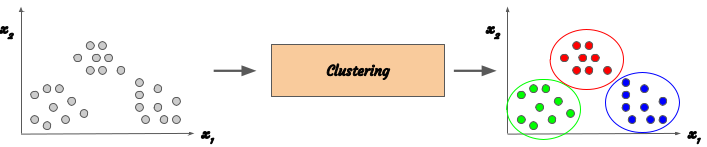
\includegraphics[width=0.6\linewidth]{imgs/17---clusetering}
    \caption{Esempio clustering}
    \label{fig:clustering}
\end{figure}



\subsubsection{Altre task}
\begin{itemize}
    \item transcription: data una immagine, descrivere con il testo
    \item machine translation
    \item anomaly detection
    \item imputation of missing value
    \item denoising
    \item density estimation
    \item synthesis
\end{itemize}

\subsection{Esperienza E}
L'esperienza è descritta da un dataset, solitamente di usa una matrice X
contenente nelle colonne tutte le features del data set(una features a colonna
, quindi ogni riga è un dato diverso).

\subsection{Labels}
Le etichette sono essenziali per fare task supervisionate, permettendo di misurare le
performance del sistema.

Possiamo assegnare ad ogni esempio una label che dice il valore corretto da predirre(Y).

\subsection{Modi per apprendere da esempi}
\begin{itemize}
    \item unsupervised learning
    \item supervised learning
    \item semi-supervised learning
    \item Reinforcement learning
\end{itemize}

Gli algoritmi non supervisionati vengono usati con dati senza label, l'algoritmo usando le features,
riesce a delineare delle classi all'interno dei dati.
Una task ricorrente nel unsupervised learning è il clustering.


Nel supervised learning, gli esempi includono un input e l'output desiderato(label), i modelli
più usati sono quello di regressione e classificazione.

semi-supervised learning, si hanno una parte di dati con le label e usando l'algoritmo si cerca di assegnare una label agli elatri elementi.



Reinforcement learning, l'esperienza non è rappresentata da un singolo dataset,
l'esperienza viene collezioanta da un "agent" che interagisce con l'ambiente, di modo
da aver un feedback loop tra il sistema e l'esperienza.

Vengono usati meccanismi di ricompensa e punizione.

\subsection{Modello di learning supervisionato}
Un modelo è uno strumento matematic che mappa l'input $X$ all'output $Y$
con la funzione $F$, dove $F$ è il modello.
I parametri si chiamano $w$.

Il modello è $y=F(X,w)$ e l'obbiettivo di ML è stimare i parametri $w$.

\subsubsection{Misura dell performance}
Una volta allenato un modello, si misura la performance(errori di classificazione
in task di classificazione o discostamento dal valore nei task di regressione).

Vogliamo sapere quato è bravo un modello a generallizzare il problema.
Per questo prima di applicare il modello, si separa il dataset in:
\begin{itemize}
    \item training
    \item test
\end{itemize}

\begin{figure}[H]
    \centering
    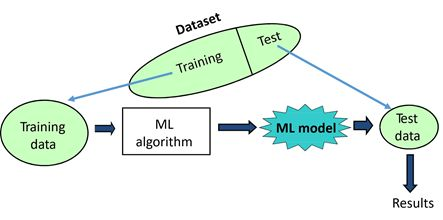
\includegraphics[width=0.5\linewidth]{imgs/18 - split}
    \caption{Split del dataset}
    \label{fig:split}
\end{figure}



\begin{figure}[H]
    \centering
    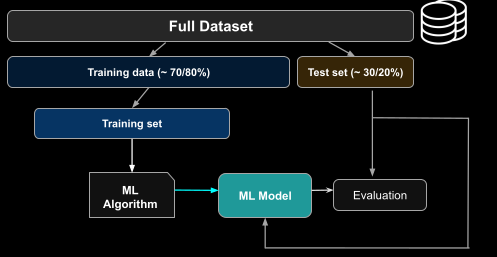
\includegraphics[width=0.5\linewidth]{imgs/19 - split2}
    \caption{Data splitting e ML}
    \label{fig:split_ML}
\end{figure}


\subsection{Loss function}
\begin{equation}
    J(w) = \frac{1}{2m}\sum_{i=1}^{m}(y_i-y_i^*)^2
\end{equation}
\begin{itemize}
    \item m è il numero di esempi
    \item $y^*$ è l'output del modello lineare
\end{itemize}
si cerca di minimizzare la loss usando delle w(parametri).

\subsubsection{Discesa del gradiente per minimizzare la loss(J)}

\begin{enumerate}
    \item abbiamo una $J(w_0,w_1)$
    \item vogliamo minimizzare J
    \item prendo una W random
    \item cerco W randomiche finchè non ottengo la J più piccola
\end{enumerate}

\begin{equation}
    W_j := \alpha\frac{d}{dW_j}J(W_0,W_1)
\end{equation}

$\alpha$ è il learning rate.

\begin{figure}[H]
    \centering
    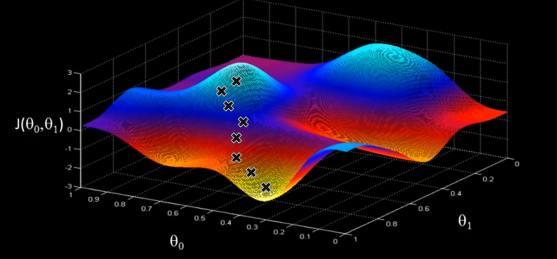
\includegraphics[width=0.5\linewidth]{imgs/discesa-gradiente}
    \caption{Discesa del gradiente}
    \label{fig:discesa_gradiente}
\end{figure}

\subsection{Discesa stocastica del gradiente(SDG)}
La discesa del gradiente è lunga e lenta perchè prende tutti i valori del
dataset, allora si usa La discesa del gradiente stocastica.

La SDG prende un'ostanza random nel training set ad ogni passo
per il calcolo del gradiente.
È più veloce.

Essendo randomica la natura del SGD, è meno regolare del gradiente normale
e migliora la discesa nella media in base alla "fortuna" del punto di
partenza.

\subsection{Regressione lineare}
Modello che fitta una linea retta.
\begin{equation}
    Y=W^{T}X
\end{equation}
Dove la $X$ è la matrice delle features e $Y$ è il vettore colonna che
contiene i target.

Calcola il gradiente cercando di ottimizzare al massimo la loss con
la linea retta.

\subsubsection{Problemi}
Avendo un modello polinomiale si può ottenere spesso un risultato migliore.

Se il data set è troppo piccolo, si tende ad andare in over fitting(il modello impara a
memoria i punti e con punti diversi va in crisi).


\subsubsection{Buonu dataset per buoni modelli}
Il modello impara dai dati $\Rightarrow$ i dati determiano la riuscita del modello.

Un buon dataset deve essere:
\begin{itemize}
    \item grande
    \item corretto
    \item consistente(esempi non contradditori)
    \item bilanciato(tutte le classi adeguatamente rappresentate)
\end{itemize}

\subsubsection{I.I.D}
Il training e il test devono essere generate da una distribuzione di probabilità.

\begin{itemize}
    \item Gli esempi nel dataset devono essere \textbf{indipendenti}
    \item il training e il test sono \textbf{identicamente distribuiti}(\textbf{I.I.D})
\end{itemize}


\subsubsection{Operfitting VS Underfitting}
\begin{figure}[H]
    \centering
    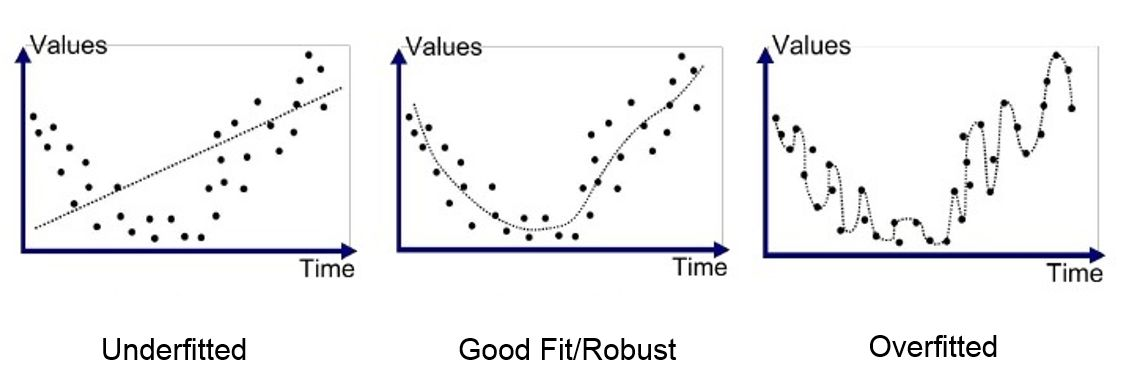
\includegraphics[width=0.6\linewidth]{imgs/underfitting_overfitting}
    \caption{Underfitting vs overfitting}
    \label{fig:under_over_fitting}
\end{figure}
Si va in \textbf{underfitting} quando un modello non riesce ad ottenere un errore
basso nel training set(probabile mancanza di dati).

Si va in \textbf{overfittin} quando gli errori nel test sono alti(probabilmente
il modello ha imparato a memoria il training).

Meglio avere un po di underfitting che overfitting, perchè nell'overfitting il modello
non è bravo a generalizzare.

\textbf{
    La chiave per è avere un errore in training basso ed
    avere il gap fra train e test basso.
}


\subsubsection{Capacità di un modello}

La capacità di un modello è l'abilità difittare una grande varietà
di funzioni.

Se ha poca capacità underfitta, se tanta capacità tende a overfittare.

Per controllare la capacità di apprendimento del modello, si usano
le \textbf{ipotesi dello spazio}(set di funzioni che il
modello può selezionare per la soluzione).


\begin{figure}[H]
    \centering
    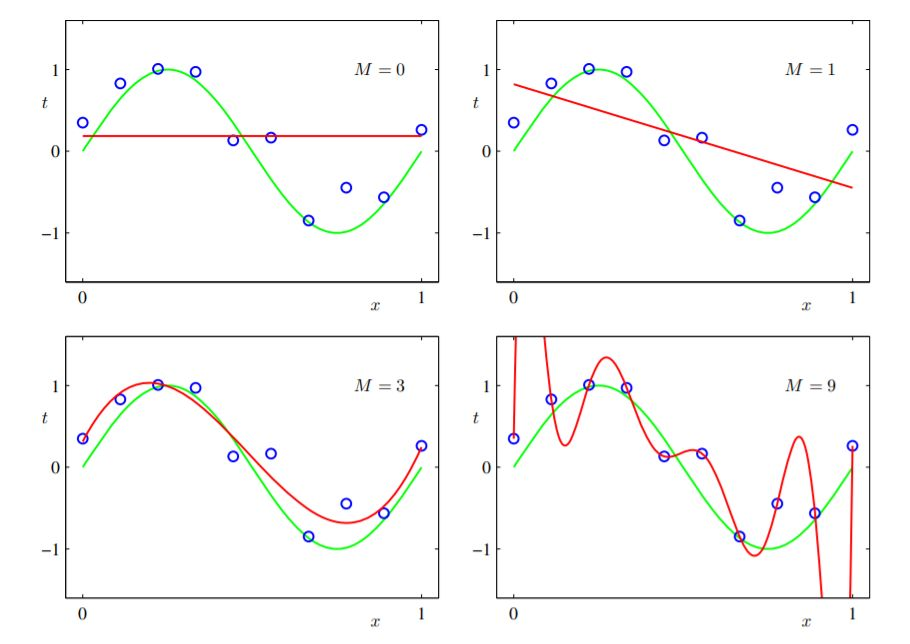
\includegraphics[width=0.6\linewidth]{imgs/ordine-polinomiale-under-over-fitting}
    \caption{Esempio di scelta del grado del polinomio}
    \label{fig:scelta_M}
\end{figure}

(regola a spanne)
Il numero di data points non dovrebbe essere meno di un x5/x10 del numero
di parametri del modello.

\subsubsection{Regolarizzazione}
Per ridurre l'overfitting, si aggiunge una penalità in termini di costo
alla funzione per scoraggiare l'overfitting.

Un aregola per la penalità semplice è la somma dei quadrati dei coefficenti:
\begin{equation}
    J(W) = \frac{1}{2m}\sum_{i=1}^{m}(Y_i-Y_i^*)^2 +
    \frac{\lambda}{2}\sum_{i=1}^{m}(W_J^2)
\end{equation}

Nel caso della regolarizzazione quadraica, prende il nome di \textbf{Ridge regression}
mentre nel neural networ si chiama \textbf{weight decay}.

\begin{figure}[H]
    \centering
    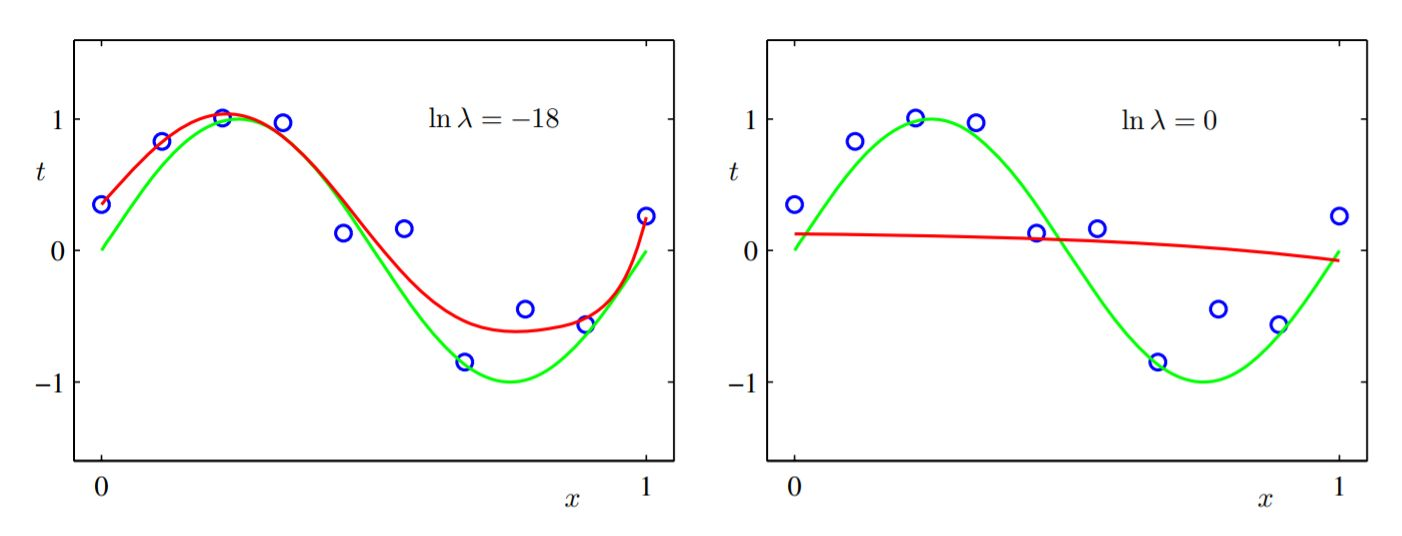
\includegraphics[width=0.5\linewidth]{imgs/esempio-lambda-regolarizzzazione}
    \caption{esempio regolarizzazione}
    \label{fig:esempio_lambda}
\end{figure}


\subsubsection{Validation set}
Il test set deve essere usato solo una volta per la vaalutazione del modello
 o modelli.

La vera division in train test e validation è:

\begin{figure}[H]
    \centering
    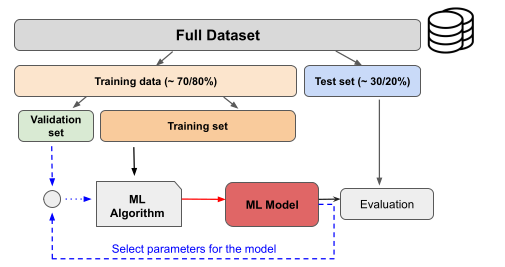
\includegraphics[width=0.65\linewidth]{imgs/train-test-validation}
    \caption{Vero train test validation}
    \label{fig:train_test_val}
\end{figure}
\begin{itemize}
    \item \textbf{training set}: dateset dove apprendere
    \item \textbf{validation set}: moddare i parametri del modello
    \item \textbf{test set}: MAI USARE, usare solo alla fine per la capacità
    di generalizzazione del modello
\end{itemize}

Ovviamente se il dataset in principio era bilanciato, ogni sotto insieme deve
essere bilanciato.











